\documentclass[a4paper]{article}
\usepackage[letterpaper, margin=1in]{geometry} % page format
\usepackage{listings,graphicx,amsmath, amssymb, amsfonts, amsthm,tikz,hyperref,fullpage,setspace,enumerate,mathtools,arydshln,pgfplots} 

\title{Homework 1}
\author{Helen Ngo}
\date{\today}

\begin{document}
\lstset{language=Python}

\maketitle

\begin {description}

\item[Problem 1.2] Consider the perceptron in two dimensions: $h(\bf x) = sign(\bf w^T \bf x)$ where $\bf w = [w_0, w_1, w_2]^T$ and $x = [1, x_1, x_2]^T$. 
\begin{enumerate}[(a)]
\item Show that the regions on the plane where $h(\bf x) = +1$ and $h(\bf x) = -1$ are separated  by a line.
\item Draw a picture for the cases $\bf w = [1,2,3]^T$ and $\bf w = -[1,2,3]^T$.
\end{enumerate}

\smallskip

\textbf{Solution:}
\begin{doublespace}
\begin{enumerate}[(a)]

\item Since $h(\bf x) = sign(\bf w^T \bf x)$ determines the classification of a point, there exits a line
\[w_0 + w_1 x_1 + w_2 x_2 = 0\]
that is in neither region and separates the two classes. Rearranging the equation of the line into the $x_2$ intercept form \footnote{Alternate form as states in the textbook: $x_2 = ax_1+b$.}, $x_2 = mx_1+b$, we have
\begin{align*}
w_2 x_2 &= -w_1 x_1 - w_0\\
x_2 &= - \frac{w_1}{w_2} x_1 - \frac{w_0}{w_2},
\end{align*}
where the slope $m = - \frac{w_1}{w_2}$ and intercept $b = - \frac{w_0}{w_2}$.

\item Let $\bf w = [1,2,3]^T$. Then $h(\bf x) = sign(\bf w^T \bf x)$
\begin{align*}
h(\bf x) &= \textbf{sign}([1,2,3]^T \bf x) \\
h(\bf x) &= \textbf{sign}(x_0 + 2x_1 + 3x_2).
\end{align*}
Therefore the slope and intercept of the line are $-\frac{2}{3}$ and $-\frac{1}{3}$ respectively.


Similarly, let $\bf w = -[1,2,3]^T$. Then $h(\bf x) = sign(\bf w^T \bf x)$
\begin{align*}
h(\bf x) &= \textbf{sign}(-[1,2,3]^T \bf x) \\
h(\bf x) &= \textbf{sign}(-x_0 - 2x_1 - 3x_2).
\end{align*}
The slope and intercept of the line are also $-\frac{2}{3}$ and $-\frac{1}{3}$ respectively. Thus both cases would have the separating line:

\begin{center}
\begin{tikzpicture}
\begin{axis}
\addplot[color=red]{-2/3*x-1/3};
\end{axis}
\end{tikzpicture}
\end{center}
\end{enumerate}
\end{doublespace}

\item[Problem 1.4] In Exercise 1.4, we use an artificial data set to study the perceptron learning algorithm. This problem lead you to explore the algorithm further with data sets of different sizes and dimensions.

\smallskip

\textbf{Solution:}
\begin{doublespace}
\begin{enumerate}[(a)]

\item Calling the perceptron learning algorithm code \cite{HB98} with

\begin{lstlisting}[frame=single]
def main():
    p = Perceptron(20)
    p.plot()
    p.pla(save=True)

main()
\end{lstlisting}

The first iteration produces a graph with a data set of size 20 with a black target function $f$ separating the red and blue classes.

\begin{center}
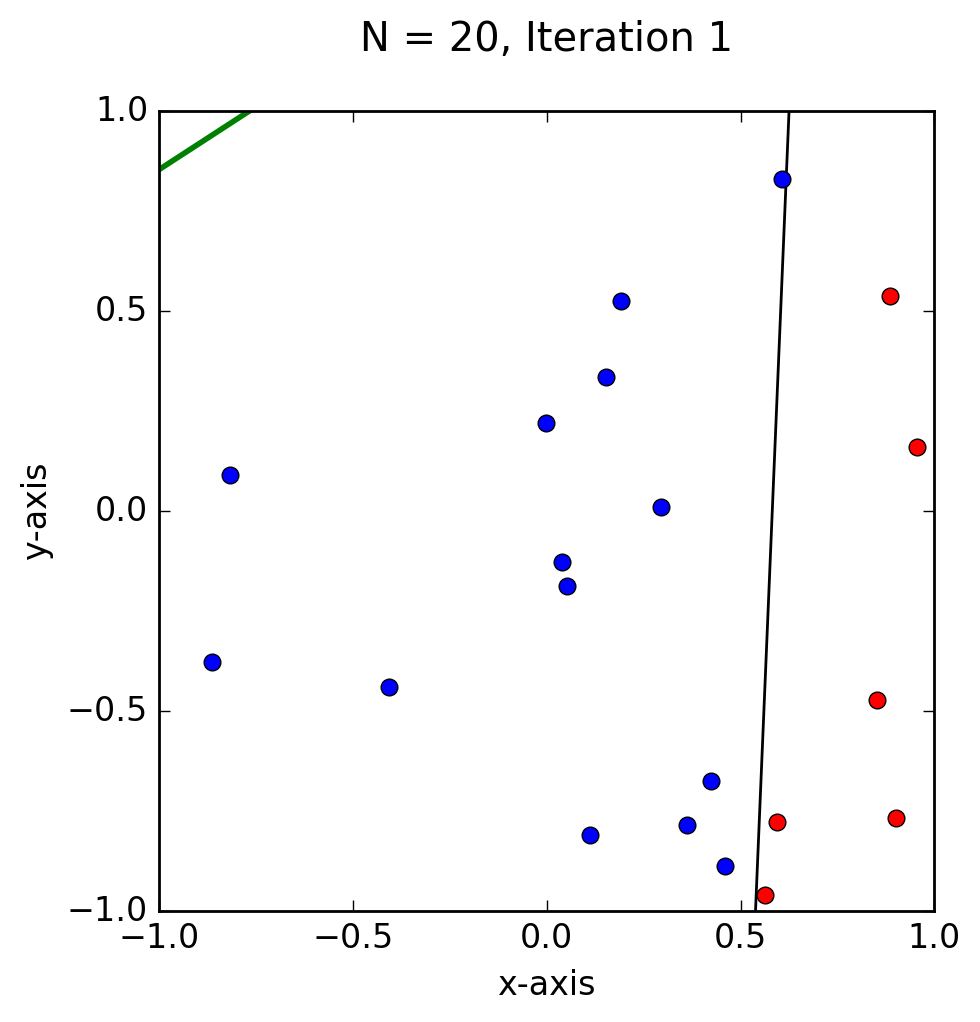
\includegraphics{Problem_4a.png}
\end{center}

\item Using the algorithm from the previous part, 33 iterations were completed before finding the final hypothesis $g$ for the same set of 20 points. The final hypothesis function is shown in green.

\begin{center}
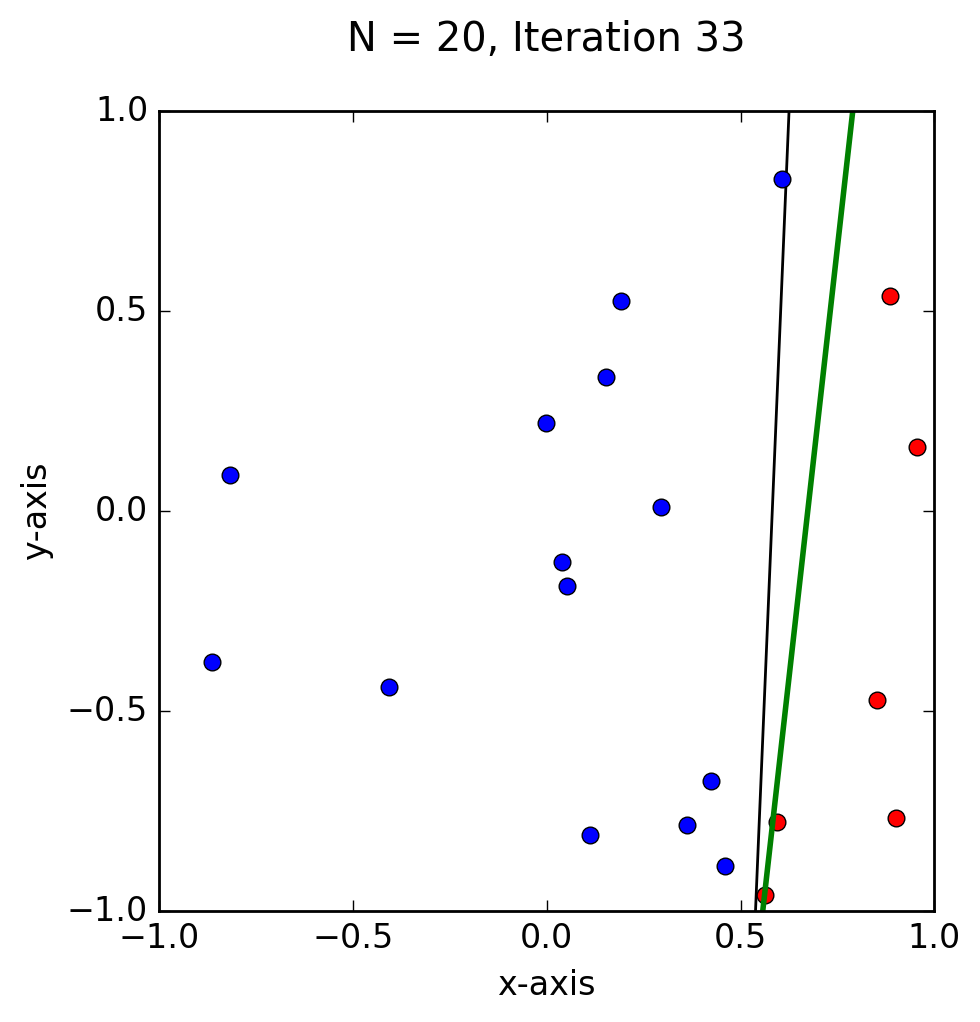
\includegraphics{Problem_4b.png}
\end{center}

Although the final hypothesis function $g$ is relatively close to the target function $f$, it should be noted that the points from the two regions are close to each other, and that all final hypothesis functions with no misclassifications would be close to the target function.

\item Running the perceptron learning algorithm again, with another randomly generated data set of size 20, the final hypothesis function $g_1$ and target function $f_1$ against the data set are shown below.

\begin{center}
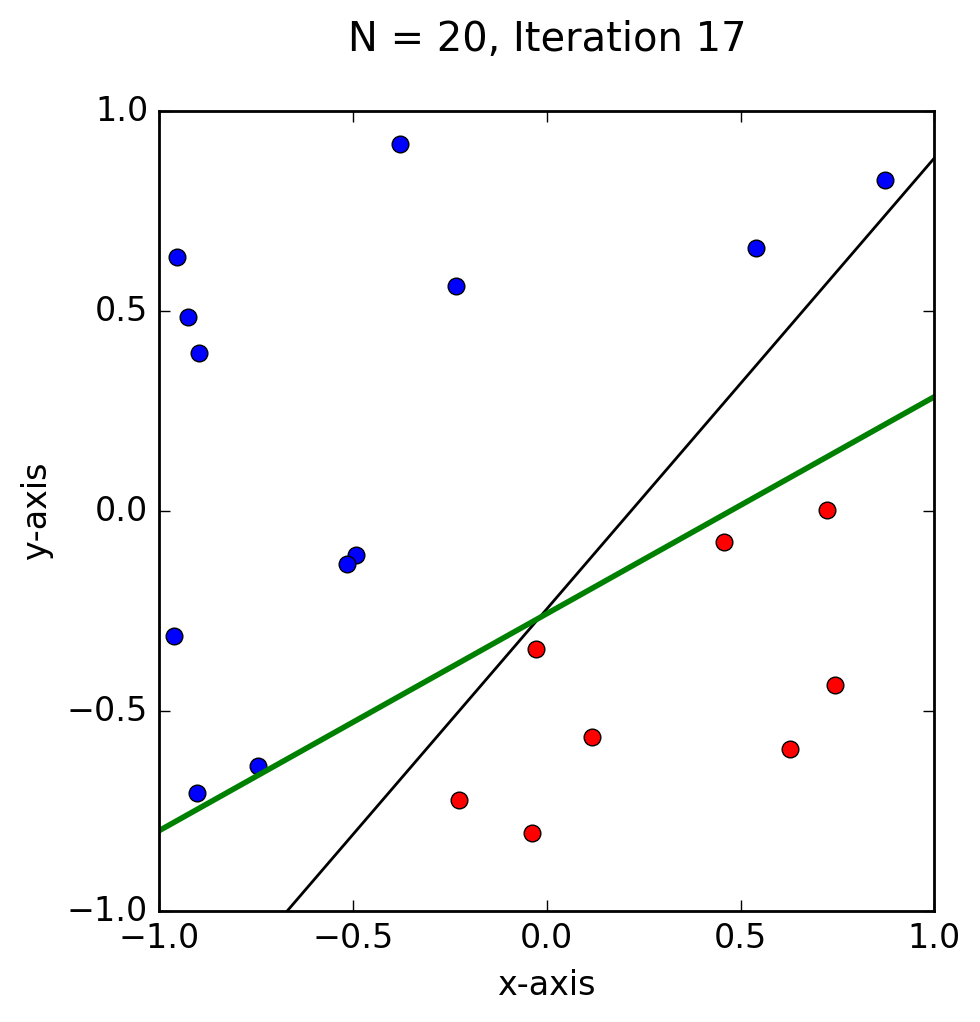
\includegraphics{Problem_4c.png}
\end{center}

It can be seen that $g_1$ is not as close to $f_1$ as $g$ is to $f$. Since the sets of data is different, it makes sense that their final hypothesis functions would have a different relationship to their respective target functions.

\item Before running the algorithm for a randomly generated data set of size 100, the ''pla" function in algorithm was modified so that only the last iteration would be saved and the iteration count printed.

\begin{lstlisting}[frame=single]
    def pla(self, save=False):
        # Initialize the weigths to zeros
        w = np.zeros(3)
        X, N = self.X, len(self.X)
        it = 0
        # Iterate until all points are correctly classified
        while self.classification_error(w) != 0:
            it += 1
            # Pick random misclassified point
            x, s = self.choose_miscl_point(w)
            # Update weights
            w += s*x
        # Plot and save the last iteration.
        if save:
                self.plot(vec=w)
                plt.title('N = %s, Iteration %s\n' \
                          % (str(N),str(it)))
                plt.xlabel('x-axis')
                plt.ylabel('y-axis')
                plt.savefig('p_N%s_it%s' % (str(N),str(it)), \
                            dpi=200, bbox_inches='tight')
        # Print iteration count.
        print(it)    
        self.w = w
\end{lstlisting}

The main function was also modified so that the perceptron generates a data set of size 100.

\begin{lstlisting}[frame=single]
def main():
    p = Perceptron(100)
    p.plot()
    p.pla(save=True)

main()
\end{lstlisting}

The experiment was repeated twice since the first trial surprisingly concluded after only 19 iterations.

\begin{center}
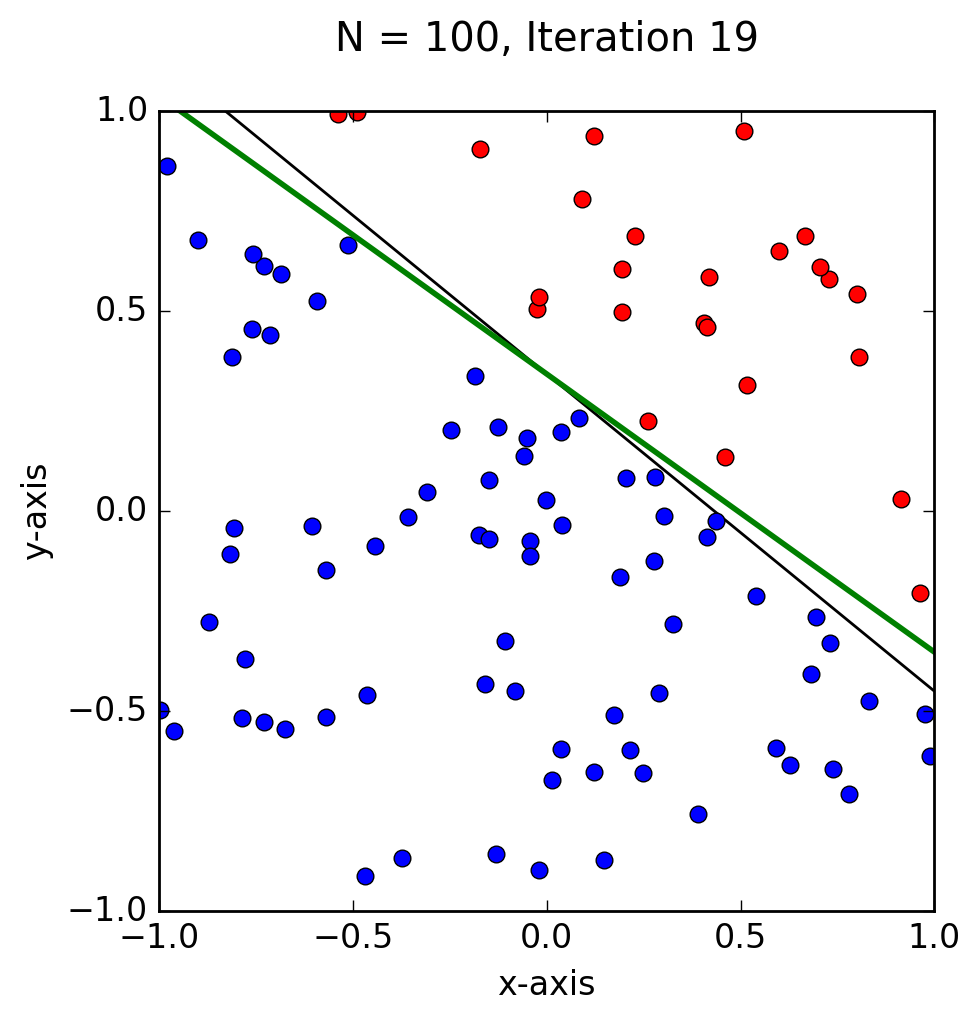
\includegraphics{Problem_4d1.png}
\end{center}

The second trial concluded after 77 iterations.

\begin{center}
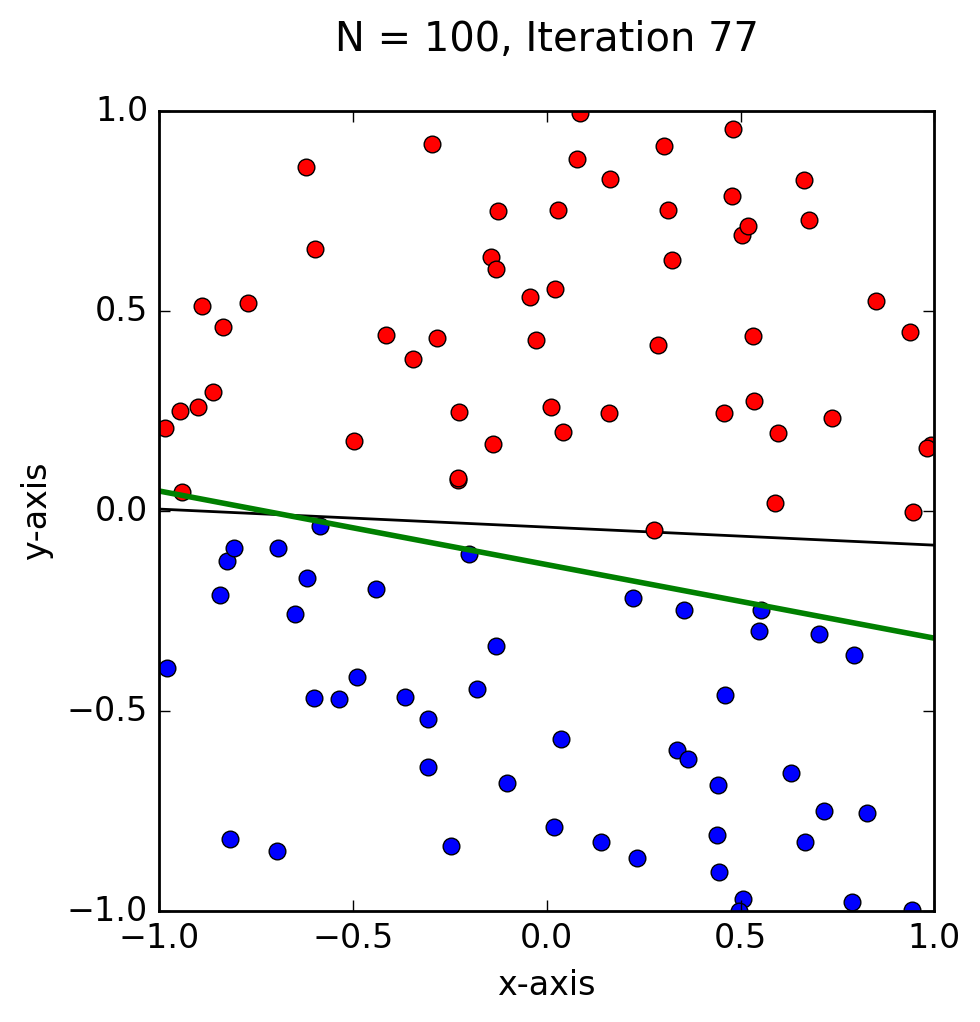
\includegraphics{Problem_4d2.png}
\end{center}

Due to the wide range of results and the small sample size of trials, it is hard to compare the results for $N=20$ to $N=100$. Based solely on these four trials, the range of iterations until the final hypothesis function is found is greater for $N=100$ than $N=20$, and it generally takes more iterations for $N=100$ to reach the final hypothesis.

\item Repeating the perceptron for 1000 randomly generated points, it took 204 iterations for the perceptron to reach its final hypothesis, which is significantly more iterations than it took the perceptron to produce the final hypothesis $g$ for $N=20$. Also, $g$ is closer to the target function than for previous sizes of data sets.

\begin{center}
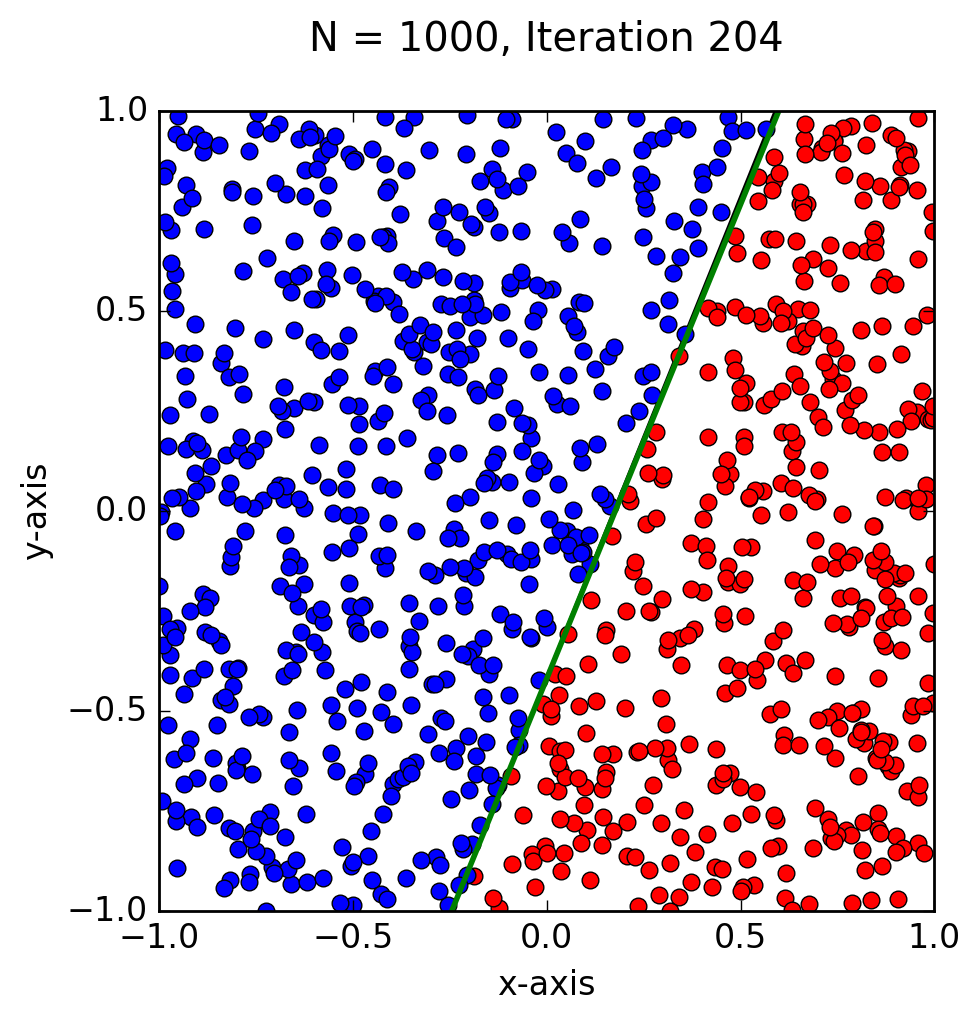
\includegraphics{Problem_4e.png}
\end{center}

\item 
\end{enumerate}
\end{doublespace}
\footnotesize
\begin{thebibliography}{99}

  \bibitem{HB98} https://datasciencelab.wordpress.com/tag/perceptron/

\end{thebibliography}
\end {description}
\end{document}
